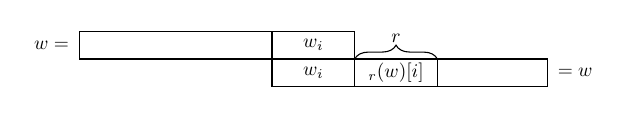
\begin{tikzpicture}[scale=0.7,every node/.style={scale=0.7}]
	\path[draw] (0,0) rectangle (3.5,0.5);
	\path[draw] (3.5,0) rectangle (5,0.5);
	\path[draw] (6.5, 0) rectangle (8.5, -.5);
	\path[draw] (3.5,0) rectangle (5,-0.5);
	\path[draw] (5, 0) rectangle (6.5, -.5);
	\draw[draw, decorate, decoration={brace,amplitude=5pt}] (5, 0) -- node[above, yshift= 5pt] {$r$} (6.5, 0);
	
	
	\node at (4.25, 0.25) {$w_i$};
	\node at (4.25, -0.25) {$w_i$};
	\node at (5.75, -0.25) {$\calS_r(w)[i]$};
	\node at (-.5, .25) {$w=$};
	\node at (9, -.25) {$=w$};
	\end{tikzpicture}